\chapter{\toolname{}}\label{chap:paynt}

\toolname{}\footnote{\url{https://github.com/gargantophob/synthesis}} (\underline{P}robabilistic progr\underline{A}m s\underline{YNT}hesiser) is a~tool to synthesise probabilistic programs automatically.
\toolname{} supports the~synthesis of finite-state programs and the~specifications given as a~conjunction of temporal logic constraints,~possibly including an~optimal objective.
The input is a~program sketch that concisely describes a~finite family of (finite) Markov chains,~and a~specification.
The tool can then identify a~family member that (potentially optimally) satisfies given specifications.
Figure~\ref{fig:sketching} depicts the workflow of \toolname{}.

\begin{figure*}[h!]
\centering
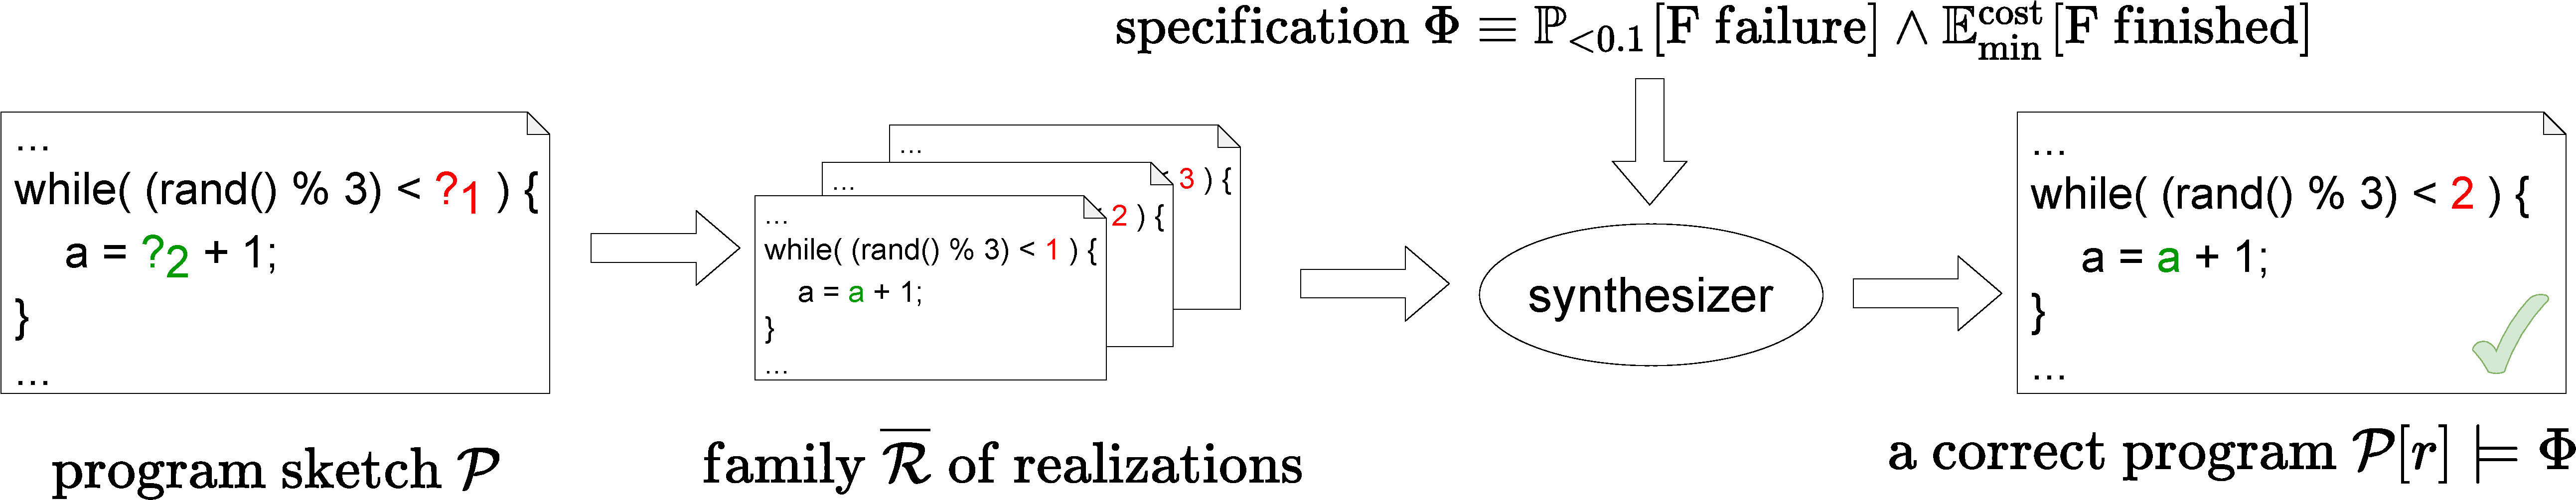
\includegraphics[width=1.0\textwidth]{figures/sketching}
\caption{The workflow of the synthesis process within \toolname{}.}%
\label{fig:sketching}%
\end{figure*}

\section{Architecture}

The design of \toolname{} is based on an~oracle-guided synthesis~\cite{tacas21} enabling a~flexible combination and integration of a~variety of state-of-the-art synthesis and verification algorithms. 
In particular,~it implements a~hybrid synthesis approach leveraging both the~\emph{CEGIS} and the~\emph{AR} oracle. 
\toolname{} is able to efficiently synthesise the~program topology (\emph{topology} synthesis) as well as continuous parameters affecting the~transition probabilities (\emph{parameter} synthesis).
Moreover,~it can handle sketches including both types of synthesis problems,~so-called a~\emph{combined} synthesis,~which is a~unique feature compering to the~existing tools. 

To achieve a high-performance synthesis, \toolname{} is implemented on top of the~probabilistic model chec\-ker \storm{}~\cite{STORM},~providing optimised verification procedures.
It is implemented in a~modular fashion on top of a~python API to provide flexibility.
\toolname{} allows to define of the~program sketches and provides all baseline synthesis algorithms under one roof.
The~tool finds application primarily for two groups of users.
First,~the~analysis of realisations sets is a~useful back-end for automated system design. %automatic engines.
For instance,~this can be used when synthesising finite-state controllers for partially observable Markov decision processes (POMDPs),~synthesising a~network protocol to increase the~packet throughput,~or selecting the~optimal power management strategy.
Second,~\toolname{} provides a modular development platform for automated design of probabilistic programs.

\begin{figure*}[h!]
\centering
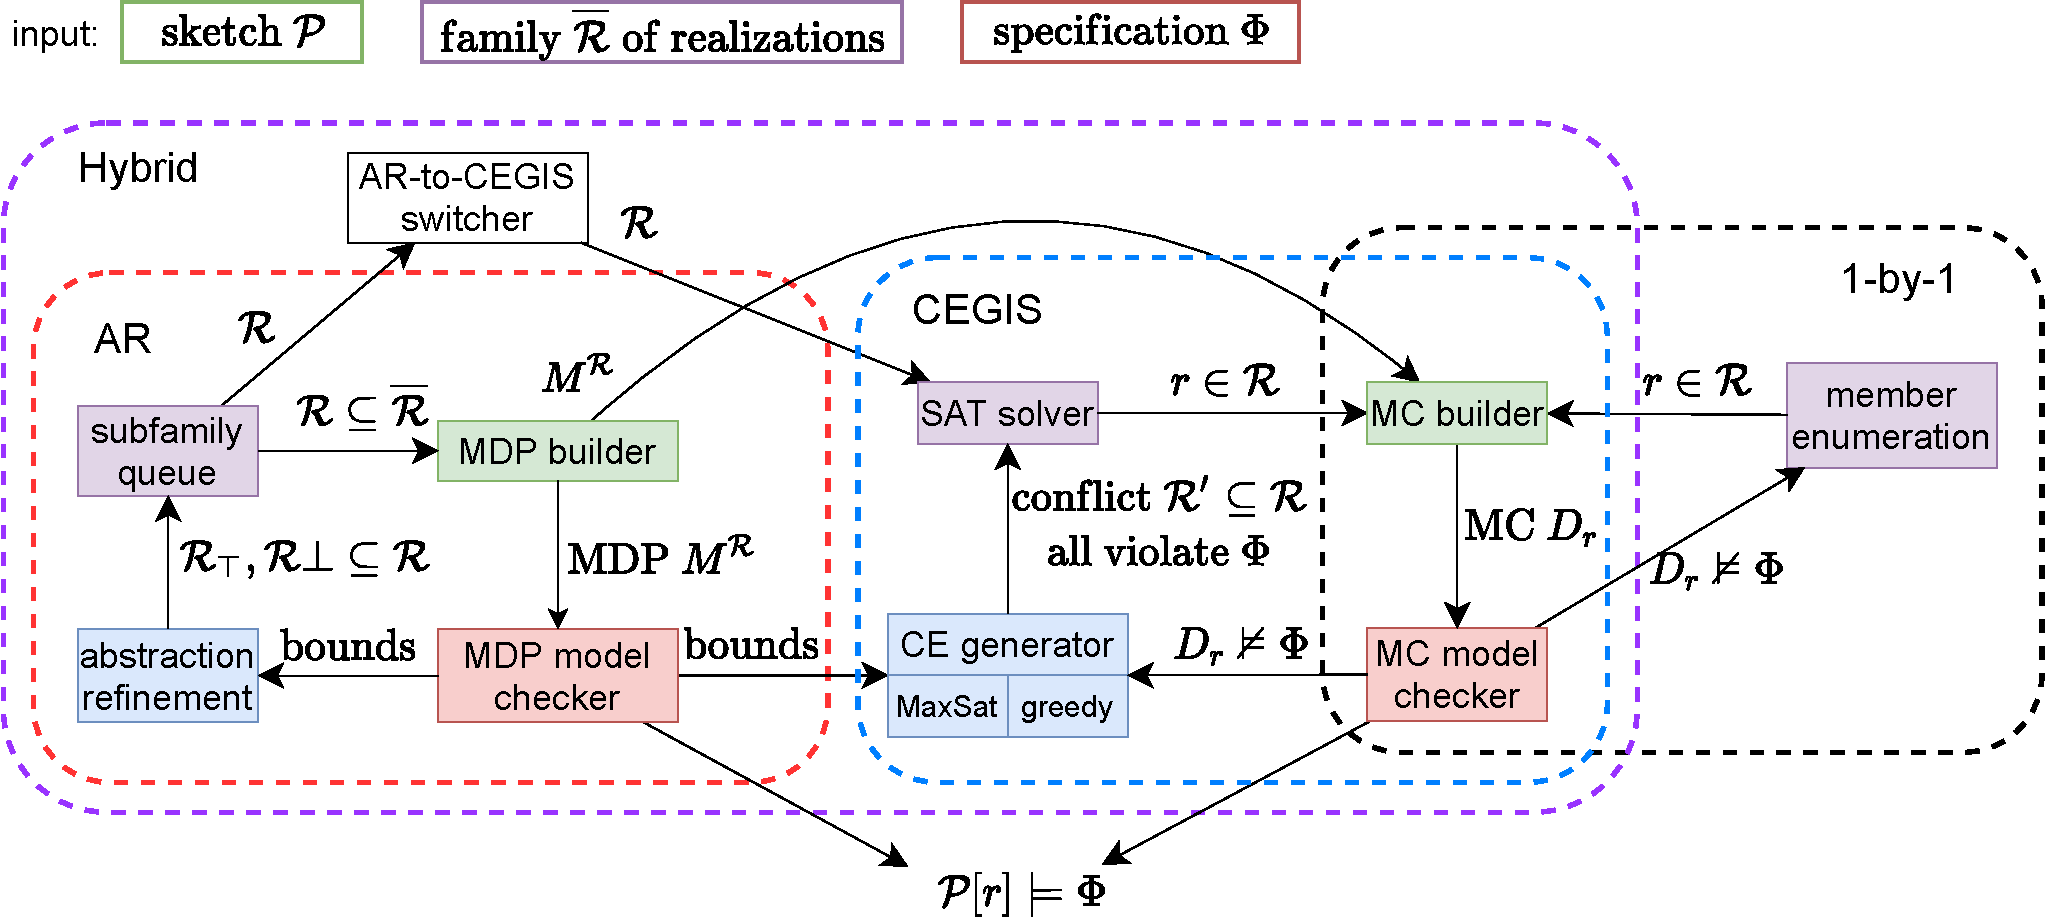
\includegraphics[width=1.0\textwidth]{figures/architecture.pdf}
\caption{The architecture of tool \toolname{}.}%
\label{fig:architecture}%
\end{figure*}

\toolname{}'s architecture (see Figure~\ref{fig:architecture}) consists of model checkers,~modules to build models and components for family handling.
The~family handlers store the~information about the~already covered design space of the~analysed family.
As the~name suggests,~the~member enumeration unit iterates over all family members.
SAT solver maintains an~SAT-formula describing undiscovered realisations,~and subsequent,~it uses Z3 SMT-solver to obtain the next candidate realisation.
The~queue with sub-families contains a~collection of unexplored sub-families refined as hyper-rectangles when the~analysis is inconclusive.
The~model builders take a~specific input according to the~active oracle and produce the~relevant model representation:
the~CE-oracle sends to the builder a single realisation $r$ while 
the~AR-oracle sends a~realisations set $\rlz' \subseteq \rlz$.
The~model checkers verify whether the constructed model (MCs or MDPs) satisfies the~given specification.
When analysing MDP,~lower and upper bounds on satisfiability probabilities are provided.
Last but not least,~\toolname{} provides a~module for generating counterexamples. In particular,~it implements two approaches: a~greedy state-expansion and a~MaxSat approach.

\paragraph{Implementation Frame.}
\toolname{} takes as the~input a~sketch written in the~\jani{} or \prism{} language and a~set of temporal properties expressed using the~PRISM syntax. 
\toolname{} is implemented on top of a~modern probabilistic model checker \storm{}~\cite{STORM} providing  high-performance verification procedures implemented in C++.
Further,~it uses Z3 theorem prover for SMT-solving and~a Python API for flexible implementation of the~synthesis loop itself.
The~implementation of \toolname{} is composed of \textit{30} Python modules containing \textit{7k} source lines of code.
We consider only our implementation and do not include extensions contributed to \storm{} and its Python API,~invoked by \toolname{}.
We tests the specific components with unit tests to maintain their correct functionality.
Regression tests verify the~accuracy and correctness of the~synthesis results and these tests currently cover more than \textit{90\%} of the~source code lines.

\section{\prism{} Sketch Language} \label{sec:pris_language}
As we said above,~\toolname{} takes as the~input the~sketch written in the~\prism{}~\cite{KNP11} or \jani{}~\cite{jani} language.
These high-level programming languages to describe probabilistic systems are more advantageous than modelling the~system as a~Markov Chain.
The~state explosion problem,~arising when using the~Markov chains as an~operational model,~renders this approach unusable.
\storm{} parses the~high-level description (sketch) written in these languages and constructs the~corresponding Markov chain,~which the~individual synthesis methods analyse.
Now,~we briefly introduce the~\prism{} sketching language proposed in~\cite{cegis}.

A~program written in \prism{} language consists of modules that interact with between itself.
We consider only programs with a~single module since more modules can be transformed into one model program.
A~module state space is given by the~set of (bounded) variables,~with their initial values and the~set of guarded commands describing the~transitions between module states.
The commands have the following form:
\begin{align*}
\texttt{[action]} \
\texttt{guard}
\ \ \rightarrow \ \
p_1 : \texttt{update}_1 + \dots + p_n : \texttt{update}_n 
\end{align*}
The~\emph{actions} ensure the~synchronisation between two or more modules when they perform the~command.
The~\emph{guard} represents a~boolean expression over the~module variables.
An~update of the~variables is selected concerning the~probability distribution defined by expressions $p_1$ through $p_n$ when guard evaluates to true.
Essentially,~the guard identifies states for which this command is applicable,~and updates describe successor states and the~probability distribution over these successors.
Overlapping of guards is disallowed since it yields non-determinism.

Moreover,~a~\textit{sketch} describes a~program containing holes representing undefined program parts that should be filled with the~value from the~finite options set.
These holes are declared as follows:
\begin{align*}
    \texttt{type} \ \texttt{hole} \ \textit{h} \ \texttt{in} \ \ \{ \mathtt{expr_1}, \dots, \mathtt{expr_k} \}
\end{align*}
The~\texttt{type} represents the domain of \texttt{hole} \textit{h} and it is an \texttt{integer} or \texttt{float}.
The~hole identifier is given by \textit{h},~and the~set of expressions $\mathtt{expr_i}$ is defined over the~program variables.
Commands and variable declarations use a~\texttt{hole} as a~component of an~\texttt{update expression} or a~\texttt{guard}.
Such a~program sketch represents a~system description with a~specified general structure but with some concrete details left out.
Instantiating all holes yields a~specific program,~and the~synthesiser target is to resolve how to substitute all holes with their options to satisfy a~given specification.
\prism{} sketching language also provides several extra functionalities: specification of the~constraints to hole values and assigning costs to option holes,~and many others.
For more detailed information,~please refer to~\cite{cegis}.

\begin{example}[\prism{} Program]
For instance,~we introduce the~following \prism{} program $\sketch$:
\begin{align*}
    & \texttt{int} \ \texttt{hole} \ \mathit{X} \ \texttt{in} \ \{ 0,1 \} \\
    & \texttt{int} \ \texttt{hole} \ \mathit{Y} \ \texttt{in} \ \{ 1,2,3 \} \\
    & \texttt{module m} \\
    & \quad \texttt{int} \ \texttt{s:} \; [0..4] \; \texttt{init} \ \texttt{X+1} \\
    & \quad [] \ \texttt{s < Y} \ \rightarrow \ \texttt{0.75}: \ \texttt{(s' = max(s-X, 0))} \ \texttt{+} \ \texttt{0.25}: \ \texttt{(s' = s+X)}; \\
    & \quad [] \ \texttt{s = Y} \ \rightarrow \ \texttt{0.50}: \ \texttt{(s' = s-1)} \ \texttt{+} \ \texttt{0.50}: \ \texttt{(s' = s+1)}; \\
    & \quad [] \ \texttt{s > Y} \ \rightarrow \ \texttt{0.25}: \ \texttt{(s' = s-1)} \ \texttt{+} \ \texttt{0.75}: \ \texttt{(s' = min(s+1, 4))};  \\
    & \texttt{end module}
\end{align*}
\label{exa:prism}
\end{example}
The~module \texttt{m} can be in one of five states: $\{ 0,1,2,3,4 \}$.
When the~module state \texttt{s} is equal to the~value of hole \texttt{Y} (\texttt{s = Y}),~it will move to the~nearest previous (\texttt{s' = s-1}) or next (\texttt{s' = s+1}) state with the~same probability of \texttt{0.50}.
When the~module state \texttt{s} is above the~value of hole \texttt{Y} (\texttt{s > Y}),~it will move to the~left neighbour with the~probability of \texttt{0.75} and with remaining to the~right if it exists,~or stay in the~last state (\texttt{s=4}).
Otherwise (\texttt{s < Y}),~the model will move the~same as in the~previous case (\texttt{X=1}),~or it stays in the~current state without change (\texttt{X=0}).
When we consider the~following instantiating of the~holes \texttt{X=1} and \texttt{Y=2},~the~corresponding underlying Markov chain is depicted below.

\begin{figure*}[h!]
\centering
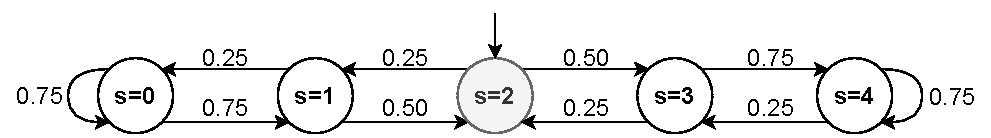
\includegraphics[width=1.0\textwidth]{figures/prism_dtmc.pdf}
\caption{An underlying Markov Chain of a probabilistic program $\sketch$ from Example~\ref{exa:prism}.}%
\label{fig:architecture}%
\end{figure*}

\section{Usage of \toolname{}} \label{sec:dpm}
We demonstrate the~usage of \toolname{} on a~synthesis problem considering a simple server for request processing depicted in Figure~\ref{fig:dpm}. 
Requests are produced by an~external unit within random intervals and maintained in a~request queue with capacity $Q_{max}$.
If the~queue is full arriving requests are lost.
The~server can operate in three modes having a different power consumption \,--\, \textit{active},~\textit{idle} and \textit{sleeping}.
The~server process the~requests only in the~\textit{active} state.
When the~server switches from a~state with low energy into a~state with higher,~extra energy is consumed,~and random latency is required.
We note that the~power consumption of request processing depends on the~current size of the~queue.
The~server operation time is finite but given as a~random process.

\begin{figure*}[h!]
\centering
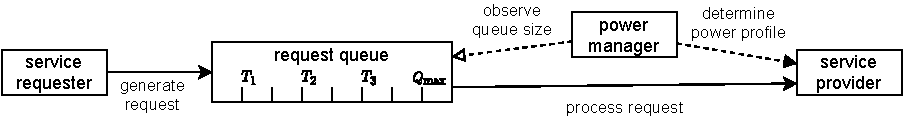
\includegraphics[width=0.9\textwidth]{figures/dpm.pdf}
\caption{The server for request processing within \emph{DPM} case study.}%
\label{fig:dpm}%
\end{figure*}

The~synthesis aims to construct a~unit called \textit{power manager} (PM),~which controls the~server.
PM observes the~current queue size and,~according to it,~then sets the~relevant power profile.
Precisely,~it differentiates between four queue occupancy levels determined by the~threshold levels $T_1,T_2$,~and $T_3$.
They indicate which fraction of the~queue capacity is currently occupied,~and they are entered into the~model as unknown parameters.
Since the~model considers three levels,~then the~power manager observers the~queue occupancy on the~following intervals: $\left[0, T_1 \right]$, $\left(T_1, T_2 \right]$, $\left(T_2, T_3 \right]$, $\left(T_3, 1 \right)$.
Moreover,~it considers a~single power profile $P_1,\dots,P_4 \in \{0,1,2\}$ for each occupancy level.
The~power profile's current value represents the~server's mode,~so the set~$\{0,1,2\}$ encodes available modes sleeping,~idle and active in the~given order.
The~following sketch describes the~module of \textit{PM}:

\begin{verbatim}
module PM
    pm  :  [0..2] init 0; // 0 - sleep, 1 - idle, 2 - active
    [sync0] q <= T1*QMAX -> (pm'=P1);
    [sync0] q > T1*QMAX & q <= T2*QMAX -> (pm'=P2);
    [sync0] q > T2*QMAX & q <= T3*QMAX -> (pm'=P3);
    [sync0] q > T3*QMAX -> (pm'=P4);
endmodule
\end{verbatim}

In this model,~we consider the~following parameters and their domains: the~queue capacity $Q_{\max} \in \{1,2,\dots,10\}$,~the~power profiles $P_1,\dots,P_4 \in \{0,1,2\}$ and the~thresholds $T_1 \in \{0.0,0.1,0.2,0.3,0.4\}$,~$T_2 \in \{0.5\}$,~$T_3 \in \{0.6,0.7,0.8,0.9\}$.
The~final sketch describing this considered model forms a~design space of $16,200$ various power managers.
The~average size of the Markov chains in this models is around $900$ states.
The~synthesis target is to find the~specific power manager,~i.e.,~the~holes instantiation,~that minimises power consumption while the~expected number of lost requests during the~server's operation time is below $1$.
We can formalise these requirements as a~pair of temporal logic formulae in the~\prism{} language:
\begin{verbatim}
R{"lost"} <= 1 [ F "finished" ]  
R{"power"}min=? [ F "finished" ]
\end{verbatim}

\toolname{} explores the~design space and produces the~following output,~including the~parameter assignment,~and the~quality value corresponds to $\Phi$ of the~analysed program:
\begin{verbatim}
QMAX=5,T1=0,T3=0.7,P1=1,P2=2,P3=2,P4=2
R[exp]{"lost"}=0.6823 [F "finished"]
R[exp]{"power"}min=9100 [F "finished"]
\end{verbatim}
The~synthesised power manager,~optimal wrt. to the~specified properties,~has the~queue capacity set to $5$ and individual thresholds at values  $1 = 0.0$, $2 = \floor{ 5\cdot 0.5}$ and $3 = \floor{ 5\cdot 0.7}$.
The~synthesised power manager performs the following strategy.
When the~request queue is empty,~then the~power manager maintains an~idle state.
Otherwise,~it always maintains an~active state,~regardless of the~exact size of the~queue,~and is never in the~sleeping state.
The~synthesised solution has a~power consumption of $9,100$ units and the~expected number of lost requests of $\approx 0.68 < 1$.

\toolname{} computes an~optimal solution in one minute. 
Although this synthesis problem is quite simple (recall it includes only 16k candidates),~\toolname{} is already $3 \times$ faster than a~naive enumeration of all realisations.
Further,~we explored a~more complex variant of this problem inspired by a~dynamical power manager's known model for complex electronic systems.
The~synthesis problem is described by the~sketch,~which covers a~family around 43M realisations.
\toolname{} solves this synthesis problem within 10~hours,~whereas the~naive enumeration takes more than one~month.

\paragraph{Combined Synthesis.}
Further,~we have expanded this model to create a~case study for combined synthesis as well.
Because of this,~we had to find some probabilistic transitions in the~system template,~which we omit and let them synthesize.
Therefore, let us first consider the following sketch described the module of a~service provider (SP):
\begin{verbatim}
module PM
    // waiting states: 3 - sleep to idle, 4 - idle to active
    sp  :  [0..4] init 0; // 0 - sleep, 1 - idle, 2 - active
    [tick1] sp <= 2 & pm <= sp -> (sp'=pm);
    [tick1] sp <= 2 & pm > sp -> (sp'=sp+3);
    [tick1] sp = 3 -> 0.8 : (sp'=sp-2) + 0.2 : true;
    [tick1] sp = 4 -> 0.6 : (sp'=sp-2) + 0.4 : true;
endmodule
\end{verbatim}
\noindent
We can see that there are states where SP has no control,~so it contains transient states ($\mathtt{sp = 3}$ and $\mathtt{sp = 4}$).
Such transient states have been introduced since a~time resolution has been considered when modelling this system to correctly model transitions with delays longer than this time resolution.
Thus,~these states are used to model the~non-unitary time transition between the~states of SP.
We decided to parameterise the~probabilistic transitions of these transient states,~which allow us to think about different time resolutions.
Therefore,~we consider the~following changes to the~SP template,~including two parameters $p_0$ and $p_1$ that affect transition probabilities:
\begin{verbatim}
    [tick1] sp = 3 -> p_0 : (sp'=sp-2) + (1-p0) : true;
    [tick1] sp = 4 -> p_1 : (sp'=sp-2) + (1-p1) : true;
\end{verbatim}
\noindent
Note that larger values of these parameters represent a~lower time resolution because the system will switch earlier between individual states.
At the~same time,~a~lower resolution time will also ensure lower power consumption.
For these parameters,~we consider intervals of length $0.2$: $p_0 \in [0.7, 0.9]$ and $p_1 \in [0.6, 0.8]$.
The~synthesis target remained unchanged,~and we are still looking for a~specific power manager that minimises power consumption,~and the~expected number of lost requests is below one.

We recall that the~considered family includes $16k$ parametric candidates compared to the~previous task of topology synthesis,~which represents a~much more difficult task due to the~continuous parameters.
\toolname{} synthesised an optimal solution in $2.8$ hours,~and the~synthesised strategy remains unchanged compared to the~presented above.
For the~sake of completeness,~we will only add that the~upper limits of the interval have been set behind the~values of the~parameters ($p_0 \approx 0.90$ and $p_1 \approx 0.8$),~which ensure the~lowest power consumption in the~lowest time resolution.
We emphasise that we have also demonstrated the correctness of the~design of our implementation for combined synthesis with this result.

